\documentclass{article}  

\usepackage[dvipsnames,table,xcdraw]{xcolor}
\usepackage{amsmath}
\usepackage{amsfonts}
\usepackage{listings}
\usepackage{lstbayes}
\usepackage{booktabs}
\usepackage{graphicx}
\usepackage{geometry}
\usepackage{pgfplots}
\usepackage{caption}
\usepackage{subcaption}
\usepackage[authoryear]{natbib}
\usepackage{float}
\usepackage{url}
\bibliographystyle{abbrvnat}
\geometry{a4paper,margin=38mm,bindingoffset=0mm,heightrounded,}

\lstset{language=R,
    basicstyle=\small\ttfamily,
%    stringstyle=\color{DarkGreen},
    otherkeywords={0,1,2,3,4,5,6,7,8,9},
    morekeywords={TRUE,FALSE},
    deletekeywords={data,frame,length,as,character},
%    keywordstyle=\color{blue},
%    commentstyle=\color{DarkGreen},
}


\DeclareMathOperator{\logit}{logit}
\DeclareMathOperator{\logistic}{logistic}
\DeclareMathOperator{\Normal}{Normal}


\linespread{1.25}


\title{Entry and line mode}
\author{Christopher M.\ Baker \and Howard Bondell \and Nathaniel Bloomfield \and Elena Tartaglia \and Andrew P.\ Robinson}
\begin{document}  
\maketitle
\begin{abstract}
In the Australian border biosecurity system, data about shipping containers is recorded in one of two modes: \emph{entry} mode or \emph{line} mode. The key difference between the modes is how the \emph{directions} are recorded, that is, data about whether entries were inspected or found to be non-compliant. In general, an entry contains multiple lines of data, where each line is a single type of item. Analysis is simple when the data is recorded in line mode: the directions are recorded individually for each line. The challenge comes when data is recorded in entry mode, because the same direction is recorded each line in the entry. In other words, if at least one line in an entry is non-compliant, then all lines in that entry are recorded as non-compliant. Therefore, entry mode data creates a challenge when we try to estimate the probability that certain items are non-compliant, because we do not know which records of non-compliance match up with which line. We develop a statistical model to use entry mode data to help inform biosecurity risk of items. We use asymptotic analysis to estimate the value of entry mode data compared to line mode data, do a simulation study to verify that we can accurately estimate parameters in a large dataset, and we apply our methods to a real dataset. 
\end{abstract}

\section{Introduction}

\paragraph{Biosecurity is important.}

\paragraph{Border biosecurity is important - pathways}
[Consider including the following here: In this paper, we assume that the outcome is either compliant or non-compliant. 
Describing non-compliance.]

\paragraph{Strategic analysis requires interception data.}

\paragraph{Cargo (volumes, activity, etc)}

\paragraph{Data capture - line and entry mode}
Data recording compliance of cargo entering Australia is recorded in two main formats: line mode and entry mode. Entry mode is often referred to as container mode in biosecurity practice, but we will only use the term entry mode in this paper for simplicity. A line is a group of the same type of item being imported. An entry is a group of lines. When cargo enters the country, each line is given \emph{directions}, which consist of a decision whether to check the line for compliance and the outcome after checking. In line mode, the directions assigned to each line are recorded along with the outcome for that line. In entry mode, directions are only recorded per entry. This means that in entry mode, if any line in that entry is found to be non-compliant, every line in that entry is recorded to be non-compliant. If all of the lines in the entry are compliant, then they are all marked compliant, so in this case line and entry mode are equivalent.

Our biosecurity data is closely related to pooled testing, which is often used for disease surveillance. Within the pooled testing literature there is generally two branches: one aims to identify positives within a pool, while the other seeks to use pooled data to estimate quantities about the population. It is the latter -- estimating quantities -- that we are interested in. The fundamental problem is estimating a prevalence, \(p\), within a population, when only pooled data is available \citep{thompson_estimation_1962}. More recent work has focussed on improving estimates by reducing bias, either through altering the sampling strategy \citep{schaarschmidt_experimental_2007,hepworth_debiased_2009} or by incorporating bias correction into models  \citep{hepworth_bias_2017,hepworth_bias_2021}. There have also been extensions of the problem where \(p\) is not a constant, but it is estimated using linear regression using only the pooled data \citep{delaigle_nonparametric_2015, chatterjee_regression_2020, mcmahan_bayesian_2017, liu_generalized_2020}. These papers have made significant progress in fitting increasingly complex models.

In practice, pooled testing is manifestly different from the biosecurity scenario. Pooled testing exists by design, as a way to gather information about a population while reducing testing. In biosecurity, the searching is done to every individual line, and the results are only pooled at the point of data capture. Hence, we are interested in how much information we are losing due to aggregating results as entry mode. Or, equivalently, how much better could we be at managing bio-security risk if we stopped using entry mode when an entry contains multiple lines?

In this paper we investigate how entry mode affects our ability to identify the biosecurity risk of items. We start with an asymptotic analysis, where we calculate the precision of estimates the implications of mixing different item types in entry mode. We then do a simulation estimation study, which allows us to understand how larger entries and more item types affect precision of estimates. Finally, we analyse a subset of Australian border interception data to see the real-world differences between using the line-only data and including the entry mode data.

\section{Model overview}\label{sec:model}
Throughout this paper, we focus on estimating the probability that a line is non-compliant, using information about it, including the type of item, country of origin and whether it has complete documentation. The full model for the probability that a line is non-compliant, \(p_{ijk\ell}\),  is: 
\begin{align}
\logit(p_{ijk\ell}) = \alpha_{i} + \beta\mathbb{I}_j + \delta_k + \gamma_\ell \label{eq:logit_model_sim},
\end{align}
where the fixed effects are $\alpha_i$, $\beta\mathbb{I}_j$ and $\delta_k$: $\alpha_i$ represents the item type, the indicator variable $\mathbb{I}_j$ denotes whether there is correct documentation, the coefficient $\beta$ is the weight given when there is correct documentation, and $\delta_k$ represents the country of provenance. The random effect $\gamma_\ell$ represents the entry effect. The indices can take values
\begin{align}
i &=1, \ldots, a, & a&\in \mathbb{N},& a &= \text{\# items}\\
j &= 1, 2, & & & &\text{without and with documentation}\\
k &= 1,\ldots, d,& d &\in \mathbb{N},& d &= \text{\# countries}\\
\ell &= 1,\ldots,g,& g&\in \mathbb{N},& g &= \text{\# entries}.
\end{align}
The values of the indicator variable are
\begin{align}
\mathbb{I}_1 & = 0,& &\text{without documentation}\\
\mathbb{I}_2 &= 1,& &\text{with documentation}.
\end{align}
The random effect $\gamma_\ell$ has distribution
\begin{align}
\gamma_\ell | \sigma &\sim \Normal(0, \sigma), & \ell &= 1,\ldots, g, & g&\in \mathbb{N}.
\label{eq:entry_effect}
\end{align}

If all data were in line mode, the above model would be a fairly standard mixed effects logistic regression with categorical variables. However, because of entry mode, we don't observe outcomes for each line, as every line in the entry is marked as non-compliant if any line in the entry is found to be non-compliant. Therefore, the outcome is whether the entry is compliant and we need to calculate the probability that the entry is non-compliant, which is 1 minus the probability that every line in the entry is compliant:
\begin{align}
\text{Entry non-compliant} = 1-\prod[1-p].\label{eq:entry_pr}
\end{align}
Hence, for entries in entry mode, we treat the entry mode as a Bernoulli random variable with probability defined by Eq.~\eqref{eq:entry_pr}, while for entries in line mode, we treat each line as a Bernoulli random variable with probability as defined in Eq.~\eqref{eq:logit_model_sim}.


This paper includes three analyses: an asymptotic analysis,
 a simulation study, and a case study of Australian biosecurity data. For the asymptotic analysis we only consider different item types, so we rather than using Eq.~\eqref{eq:logit_model_fit_sim}, we just consider the probability that a line of item type \(i\) is non-compliant, \(p_i\). The simulation study and the case study both use the full model, as defined above. 


\section{Asymptotic analysis}
We use asymptotic analysis to investigate how the precision of estimates depends on entry size, the number of entries, the probability of interception and whether item types are mixed. This analysis is broken into two parts. The first part assumes that all items are a single type, which allows us to quantify how the amount of data, probability of interception and entry size affects precision. The second part assumes that there are two different item types, and it explores how changing the proportion of entries with both item types mixed affects precision.

Throughout this section we make two simplifications. Firstly, we do not separate line mode and entry mode because entry mode data with entry size 1 is mathematically equivalent to line mode data. Hence, throughout these analysis, entry size 1 means line mode and entry size greater than 1 implies entry mode. Secondly, we  assume that each item has a fixed probability of interception. Therefore, we consider each line a Bernoulli trial, which only depends on the item type. When the entry size is greater than one, the relevant probability is whether at least one line was intercepted.

We estimate precision via calculation the Fisher information matrix, \(\mathcal{I}\). The Fisher information  matrix is the expected value of the negative of the Hessian matrix of the log-likelihood evaluated at the value of the parameter. We use the standard error estimate as our measurement of precision, which are the square roots of the diagonal elements of the inverse of \(\mathcal{I}\).

\subsection{Single item type}
For the single item type case, we set the probability of interception to be \(p\), and define \(N\) as the total number of entries, \(I\) as the number of entries intercepted and \(S\) as the size (i.e. the number of lines) in each entry. The likelihood is a binomial distribution, where the outcome is the an entry being intercepted. The probability that an entry is not intercepted is
\begin{align}
\mathbb{P}(\text{entry not intercepted}) = (1-p)^S,
\end{align}
meaning that the binomial likelihood for a set entry size, S, is
\begin{align}
\mathcal{L}_S = \left(1-(1-p)^S\right)^I\left(1-p)^S\right)^{N-I}. \label{eq:entry_mode_like}
\end{align}
To generalise Eq.~\eqref{eq:entry_mode_like} to arbitrary entry sizes, we need the product over entry size:
\begin{align}
\mathcal{L}& = \prod_{S\in\mathbb{N}} \left(1-(1-p)^S\right)^{I_{E,S}}\left((1-p)^S\right)^{N_{E,S}-I_{E,S}},
\label{eq:aymptotic_full_likelihood}
\end{align}
where \(S\) is the entry size, \(I_{E,S}\) is the number of inteceptions of entry size \(S\) and \(N_{E,S}\) is the number of entries of size \(S\).  The log-likelihood is
\begin{align}
\log\mathcal{L}& = \sum_{S\in\mathbb{N}}{I_{E,S}} \log\left(1-(1-p)^S\right)+(N_{E,S}-I_{E,S})\log\left((1-p)^S\right).
\label{eq:loglikelihood_arbitrary_entry_size}
\end{align}
As there is only one parameter, we calculate its second derivative rather than there being a Hessian matrix:
\begin{align}
\left[\frac{\partial^2 \log\mathcal{L}}{\partial p^2}\right]= \sum_{S\in\mathbb{N}}
\frac{S\left(N_{E,S} + \frac{I_{E,S}((1+S)(1-p)^S-1)}
{\left((1-p)^S-1 \right)^2} \right)}
{(1-p)^2}.\label{eq:loglike_2nd_deriv}
\end{align}
To calculate the Fisher information, we need the expected value of the number of interceptions, which depends on the size of the entry:
\begin{align}
\mathbb{E}\left[I_{E,S}\right] = N_{E,S}(1-(1-p)^S). \label{eq:exp_intercept}
\end{align} 
Hence the Fisher information is
\begin{align}
\mathcal{I} = -\mathbb{E}\left[\frac{\partial^2 \log\mathcal{L}}{\partial p^2}\right]=
 -\sum_{S\in\mathbb{N}}\frac{N_{E,S}S^2(1-p)^{S-2}}{(1-p)^S-1}, \label{eq:fisher_information}
\end{align}
and the standard error estimate is
\begin{align}
SE = \sqrt{\frac{1}{-\sum_{S\in\mathbb{N}}\frac{N_{E,S}S^2(1-p)^{S-2}}{(1-p)^S-1}}}.\label{eq:general_SE_calc}
\end{align}


Using Eq.~\eqref{eq:general_SE_calc} we can understand how the probability of interception, the entry size and the number of lines affect the standard error, and we plot these relationships in Figure~\ref{fig:asymptotic_SE_plots}. The left plot shows that the standard error depends on the probability of interception and that the relationship depends on the entry size. For all entry sizes, the standard error is small when the probability of interception is small (below \(\sim 0.3\)). However, for larger values of the probability of interception, the standard error increase significantly if the entry size is three or greater. The large \(p\) behaviour is driven by the \((1-p)^{S-2}\) term in Eq.~\eqref{eq:general_SE_calc}, which means SE goes to 0 if \(S=1\), while it diverges if \(S\geq 3\). Figure~\ref{fig:asymptotic_SE_plots} also shows how the standard error decreases as the number of lines of data increases. The lower the entry size is, the lower the standard error, and, as \(SE\sim\sqrt{1/N_{E,S}}\), entry mode data with larger entry sizes require a large amount of data to reach the same standard error. 


\begin{figure}[h!]
\begin{subfigure}[b]{0.49\textwidth}
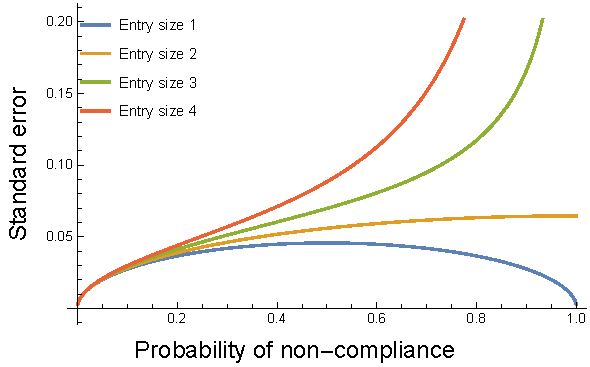
\includegraphics[width=\textwidth]{../asymptotic_approximation/SE_vs_pr_intercept.pdf}
\end{subfigure}
\hfill
\begin{subfigure}[b]{0.49\textwidth}
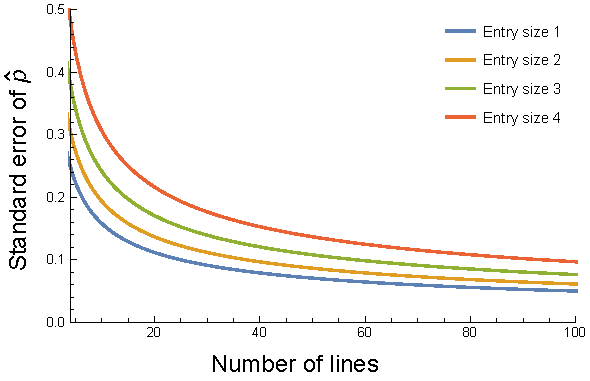
\includegraphics[width=\textwidth]{../asymptotic_approximation/SE_vs_num_lines.pdf}
\end{subfigure}

\caption{The standard error (Eq.~\eqref{eq:general_SE_calc}) as the probability of interception, \(p\), is varied (left) and as the number of lines are varied (right). For the left plot the number of lines is held constant at 120. For the right plot, the probability of interception is held constant at 0.5}
\label{fig:asymptotic_SE_plots}
\end{figure}


\subsection{Two item types}
In this section we consider a situation where there are two items with probabilities of interception of \(p_1\) and \(p_2\), and we examine how these different items type probabilities interact. We focus on a scenario where every entry is of size two, meaning there are three types of entries: only type 1; only type 2; or mixed, with one line of type 1 and one of  type 2. We denote the number of lines within a single entry of type 1 and 2 as \(S_1\) and \(S_2\) respectively, and \(I(S_1,S_2\) and \(N(S_1,S_2)\) are the number of interceptions and total number of entries with \(S_1\) type 1 lines and \(S_2\) type 2 lines. For our case, we can have \(S_1=2, S_2=0\), \(S_1=1, S_2=1\) or \(S_1=0, S_2=2\). Rewriting the log-likelihood from Eq.~\eqref{eq:loglikelihood_arbitrary_entry_size}, we get
\begin{align}
\log\mathcal{L} = \sum_{S_1,S_2}{I(S_1,S_2)}\log\left(1-(1-p_1)^{S_1}(1-p_2)^{S_2}\right) + (N(S_1,S_2)-I(S_1,S_2))\log\left((1-p_1)^{S_1}(1-p_2)^{S_2}\right). \label{eq:entry_mode_loglike_2types}
\end{align}
We compute the Fisher information matrix and the standard error using Mathematica. The standard error for \(p_1\) is

\begin{align}
\frac{1}{2} \sqrt{-\frac{{p_1} \left(p_1^2-3 p_1+2\right) (N_{1,2} (p_1-1) (p_2-2) p_2+4 N_{2,2} (p_2-1) (p_1 (p_2-1)-p_2))}{N_{1,1} (p_1-1) (N_{1,2} (p_1-1) (p_2-2) p_2+4 N_{2,2} (p_2-1) (p_1 (p_2-1)-p_2))+N_{1,2} N_{2,2} (p_1-2) p_1 (p_2-1)^2}},\label{eq:p1_two_type_SE_est}
\end{align}
where \(N_{1,1}\) and \(N_{2,2}\) are the number of entries with two type 1 lines and two type 2 lines respectively, while \(N_{1,2}\) are the number of entries with both type 1 and type 2 lines. The standard error for \(p_2\) is the same, with \(N_{1,1}\) and \(N_{2,2}\) switched and \(p_1\) and \(p_2\) switched. 

By examining Eq.~\eqref{eq:p1_two_type_SE_est} we can see that the behavior of the standard errors is more complex than when we considered only one type of item. Notably, the number of entries of only type 2, \(N_{2,2}\), is in the equation for the type 1 standard error, along with the probability of interception of type 2, \(p_2\). 

Figure~\ref{fig:two_type_se_fourplot} shows how the standard error varies with the proportion of mixed entries, for different interception probabilities. In each case, we hold \(p_1\) at 0.1, and we vary \(p_2\) for 0.05 up to 0.9 across the four plots. Interestingly, how the standard error changes as a function of the proportion of mixed entries changes markedly, depending on the value of \(p_2\). In particular, when \(p_2\) is 0.7 and 0.9, the standard error for the \(p_1\) increases as the proportion of mixed entries increases, while the standard error for \(p_2\) actually decreases, while the proportion of mixed entries is below \(\sim 90 \%\).



\begin{figure}[H]
\begin{subfigure}[b]{.49\textwidth}
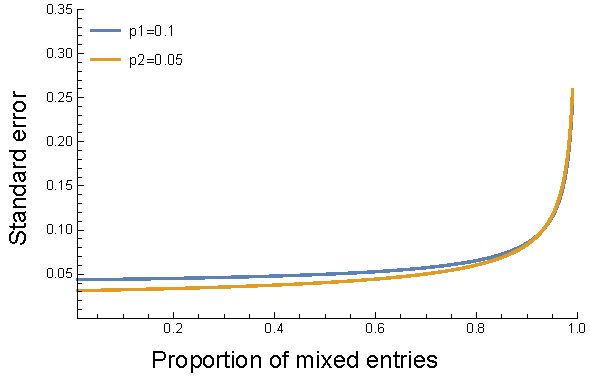
\includegraphics[width=\textwidth]{../asymptotic_approximation/SE_twotype_p1_01_p2_005.pdf}
\end{subfigure}
\hfill
\begin{subfigure}[b]{0.49\textwidth}
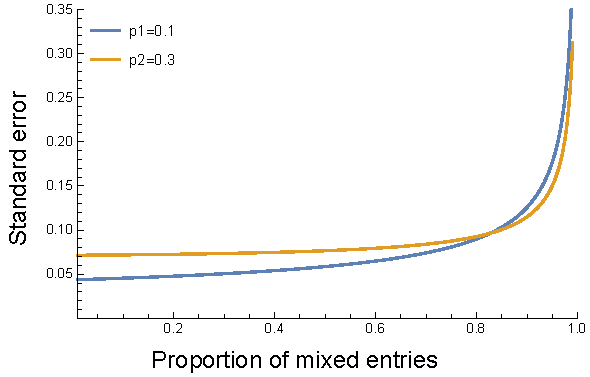
\includegraphics[width=\textwidth]{../asymptotic_approximation/SE_twotype_p1_01_p2_03.pdf}
\end{subfigure}
\hfill
\begin{subfigure}[b]{0.49\textwidth}
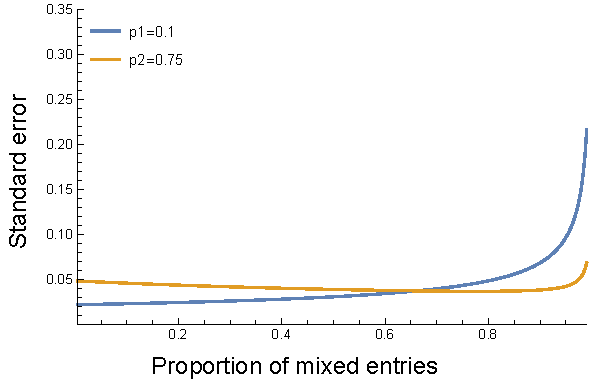
\includegraphics[width=\textwidth]{../asymptotic_approximation/SE_twotype_p1_01_p2_075.pdf}
\end{subfigure}
\begin{subfigure}[b]{0.49\textwidth}
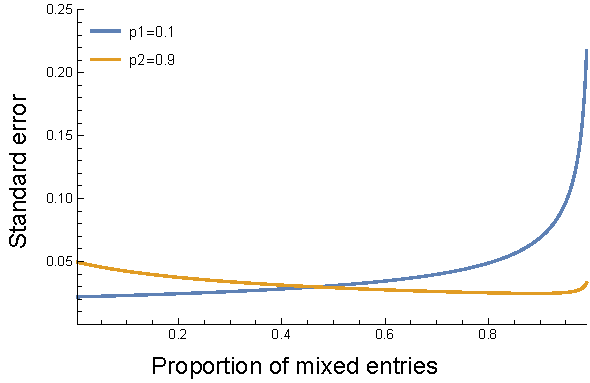
\includegraphics[width=\textwidth]{../asymptotic_approximation/SE_twotype_p1_01_p2_09.pdf}
\end{subfigure}

\caption{The standard error when for entry size 2, when the proportion of mixed entries is varied. In each plot there are 50 total entries and \(p_1\) is held constant at 0.1, while \(p_2\) goes from 0.05 up to 0.9.}
\label{fig:two_type_se_fourplot}
\end{figure}

%
%Across the plots in Figure~\ref{fig:two_type_se_fourplot}, the behavior of the standard error for \(p_1\) looks quite similar. However, comparing the standard error for \(p_1\) for different values of \(p_2\) shows that the value of \(p_2\) has a measurable impact on the standard error of the \(p_1\) estimate (Figure~\ref{fig:two_type_p1_fixed_p2_vary}). Here we see that the standard error for \(p_1\) increases as the value of \(p_2\) increases. Combing this result with the results in Figure~\ref{fig:two_type_se_fourplot}, we see that if low and high probability items are mixed in entry mode, we can estimate the risk of the high probability items, but it comes at the detriment for our ability to identify low-risk items. 
%
%
%
%\begin{figure}[H]
%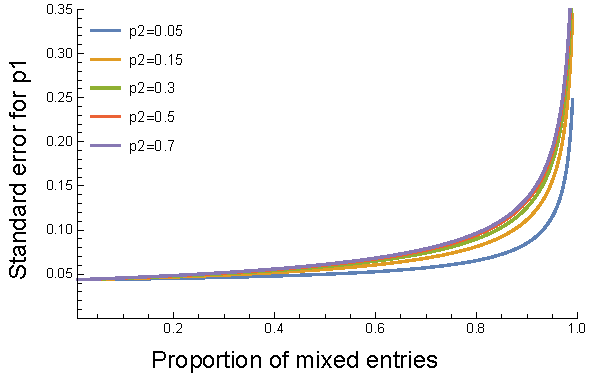
\includegraphics[width=.65\textwidth]{../asymptotic_approximation/SE_twotype_p1_p2_range.pdf}
%\caption{The stand error for \(p_1\) as the proportion of mixed entries changes for varying \(p_2\). The number of total entries is held constant at 50.}
%\label{fig:two_type_p1_fixed_p2_vary}
%\end{figure}


\subsection{Asymptotic analysis conclusions}

From the asymptotic analysis we can conclude two key lessons:
\begin{enumerate}
\item Entry mode data is most useful when the probability of interception, \(p\), is small. In the extreme case where \(p\rightarrow 0\), entry mode data is equivalent to line mode data because whenever an entry is \emph{not} intercepted, we know every line was not intercepted, regardless of whether it is entry mode or line mode. 
\item When \(p\) is not small (e.g. greater than 0.5) it can still be useful to analyse entry mode data, but only if the amount of line mode data is small. However, if there is sufficient line mode data to get acceptable precise parameter estimates, there would be little to gain by using entry mode data.
\item Entries in entry mode with mixed entries can increase or decrease the precision of estimates, depending on the true probability of interception. If the probability of interception is low, mixed entries tend to lead to lower precision, but item types with high probability of interception may lead to lower standard errors.
\end{enumerate}


\section{Simulation study}
As the first step in developing a method to analyse real-world data sets, we simulate a data set that contains key complexities including multiple item types, fixed effects and random effects. Once we have simulated data, we can fit a model to estimate parameters. The advantage of our approach is that we can (1) verify that our model behaves correctly and (2) explore how model precision varies in a more complex setting.

\subsection{Data simulation}
We simulate data from the full model (as described in Section~\ref{sec:model}). For our simulations, chose parameters which we expect to be similar to their values in real-world data. We set \(\beta=-1\), choosing an negative effect of having correct documentation, because we expect lines with correct documentation have a higher chance of being compliant. We include $a=5$ item types with \(\alpha_i\) taking values of -6.91, -4.60, -3.89, -2.94, -1.39 (corresponding to interception probabilities of 0.001, 0.01, 0.02, 0.05 and .2, if all other effects were 0). We chose negative values for the item effect $\alpha_i$, since the probability of detection is expected to be low for any item in real-world data. We used $d=3$ countries and choose their weights to be .5, -1 and .25, {\color{red} because\ldots}
{
\color{red}
We run simulations with and without an entry effect, but when we include entry \eqref{eq:entry_effect} it takes a normal distribution with mean zero and standard deviation \(\sigma = 0.25\). For each entry we draw whether it is in line mode or not with probability 0.25, and for each line we set the probability of having correct documentation to be 0.2.}

{\color{red} Do we need to specify how we generated values for countries and entries?}  

We show an example of the format of the data in Table \ref{table:example_data}.

\vspace{0.1cm}
\begin{table}[h]
\caption{Example simulated data. Lines 1-3 are all marked as intercepted because entry 1 is in entry mode, even though only 1 or 2 of the lines were actually intercepted.}
\label{table:example_data}
\begin{center}

\begin{tabular}{|c|c|c|c|c|c|}
\hline 
Line & Entry & Type & Documentation & Mode & Intercepted \\ 
\hline 
1 & 1 & 3 & 1  & Entry & 1 \\ 
\hline 
2 & 1 & 2 & 0  & Entry & 1 \\ 
\hline 
3 & 1 & 1 & 0 & Entry & 1 \\ 
\hline 
4 & 2 & 5 & 0 &Line & 0 \\ 
\hline 
5 & 3 & 4 & 1 &Line & 1 \\ 
\hline 
\vdots & \vdots & \vdots & \vdots & \vdots & \vdots \\ 
\hline 
\end{tabular} 

\end{center}
\end{table}

\subsection{STAN model}
We model the system in a Bayesian framework, using the RSTAN package in R. The basic structure for fitting the simulated data is to define the probability of interception for each line (following Eq.~\eqref{eq:logit_model_sim})
\begin{align}
\logit(p_{ijk\ell}) = \alpha_{i} + \beta\mathbb{I}_j + \delta_k + \gamma_\ell, \label{eq:logit_model_fit_sim}
\end{align}
where 
\begin{align}
\gamma_\ell | \sigma &\sim \Normal(0, \sigma), & \ell &= 1,\ldots, g, & g&\in \mathbb{N}.
\end{align}
As we fit our model in a Bayesian framework, we set priors on each parameter:
\begin{align}
\alpha_i &\sim \Normal(-4, 4), & i&=1, \ldots, a, & a&\in \mathbb{N},\\
\beta &\sim \Normal(0, 0.5),\\
\delta_k &\sim \Normal(0, 0.5), & k &= 1,\ldots, d, & d &\in \mathbb{N}\\
\sigma &\sim \Normal(0, 0.5)
\end{align}

The probability $p_{ijk\ell}$ is the probability of non-compliance of a line that has characteristics $(i,j,k,\ell)$. We denote the probability that line $n$ is non-compliant as $p_{(n)}$, where $p_{(n)} = p_{ijk\ell}$ if that line has characteristics $(i,j,k,\ell)$.

%If the data were exclusively in line mode, fitting the model would be relatively standard, as it is logistic regression. For the line mode data, the random variable that indicates whether line $n$ is non-compliant has a Bernoulli distribution
%\begin{align}
%\text{Non-compliant}_{n, \text{line}} \sim \text{Bernoulli}(p_{(n)}).
%\end{align}
%
%However, the entry mode data complicates the model, because for each entry there is only one response variable, irrespective of how many lines are contained within the entry. Hence, as we did in the asymptotic analysis for the entry data (Eq.~\eqref{eq:entry_mode_like}), we need to calculate the probability that at least one line in the entry is non-compliant:
%\begin{align}
%\mathbb P(\text{Entry } \ell \text{ non-compliant}) = q_\ell = 1 - \prod_{n\in\text{lines}(\ell)} (1-p_{(n)}),
%\end{align}
%where $\text{lines}(\ell)$ is the set of all lines in entry $\ell$.
%
%Therefore, for entry mode data, the random variable that indicates whether entry $\ell$ is non-compliant has distribution
%\begin{align}
%\text{Non-compliant}_{\ell, \text{entry}} \sim \text{Bernoulli}(q_\ell).
%\end{align} 
%{
%\color{red}
%Why are we talking about the distributions of these random variables in the STAN model section?
%}{\color{blue} this defines the likelihood}
%
%\subsection{Model verification}
%The primary aim of our work is to investigate the relative contribution of entry mode data to precision of parameter estimates. However, before analysing precision it is important to ensure that we are able to accurately estimate parameters with our model and that precision estimates using STAN match the asymptotic analysis.
%\subsubsection{Model precision}
%To check model precision, we simulate a simplified dataset, with a single item type and no other fixed or random effects, and compare the STAN estimates with the asymptotic approximation, from Eq.~\eqref{eq:general_SE_calc}. As STAN is a Bayesian approach, it is apropriate to comapare the standard error estiamte, Eq.~\eqref{eq:general_SE_calc}, to the standard deviation of the STAN posterior draws. 
%The simulation uses \(p=0.05\) and we vary the number of entries \(N_E\) and the entry size, \(S\) and the comparison is shown in Figure~\ref{fig:SD_est_simulated}.

\subsection{Simulation results}

\begin{figure}[h!]
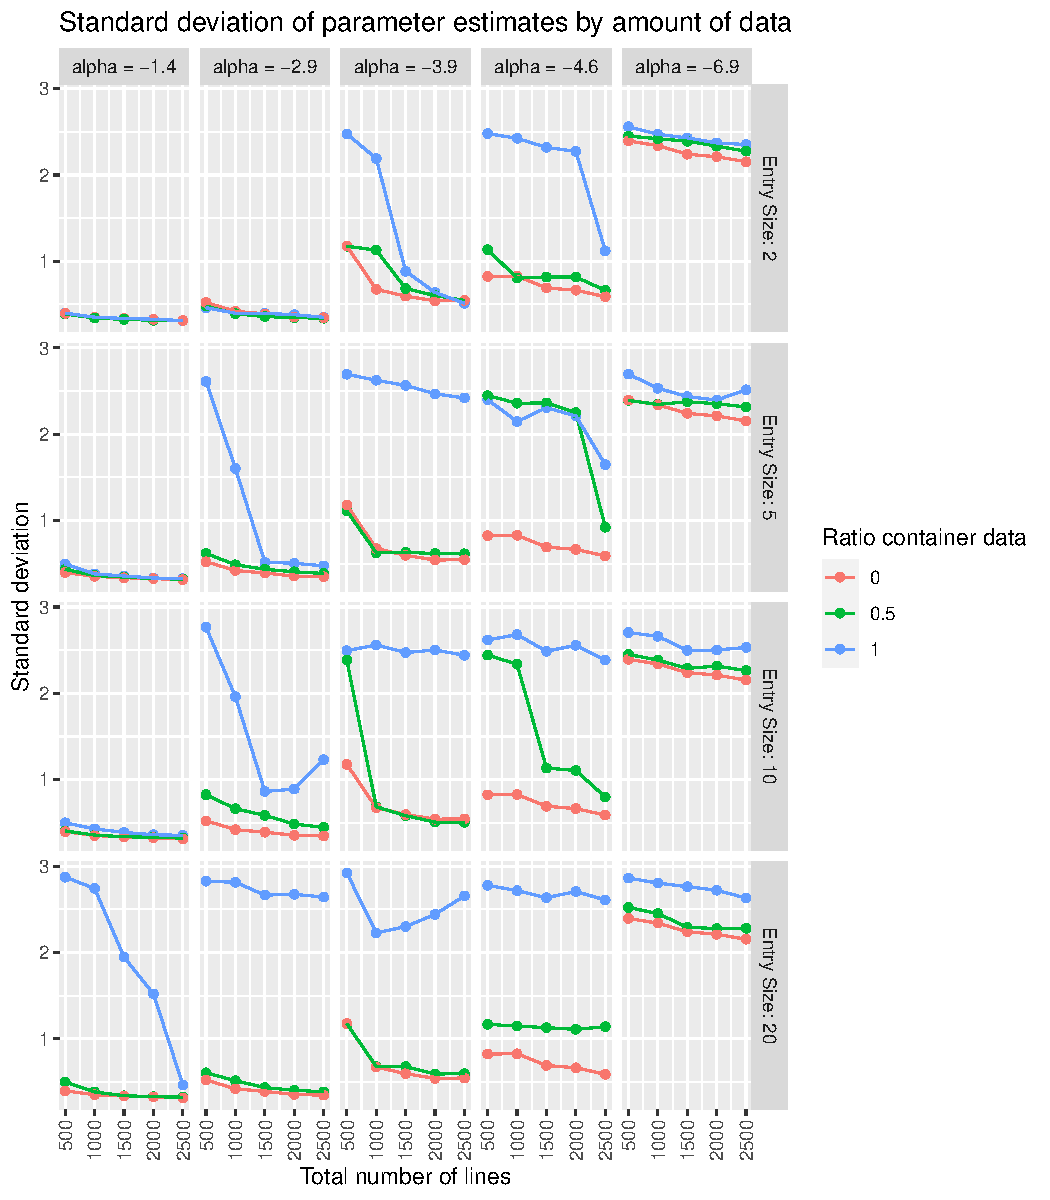
\includegraphics[width=\textwidth]{../visualisations/figures/sim_study_pint_vs_data_vs_entry_size.pdf}
\caption{SD as amount of data increases, depending on \(p\) and the amount of entry data}
\label{fig:SD_est_simulated}
\end{figure}




\section{Case study}
We use border interception data from Australia to compare the diff



\begin{figure}[h!]
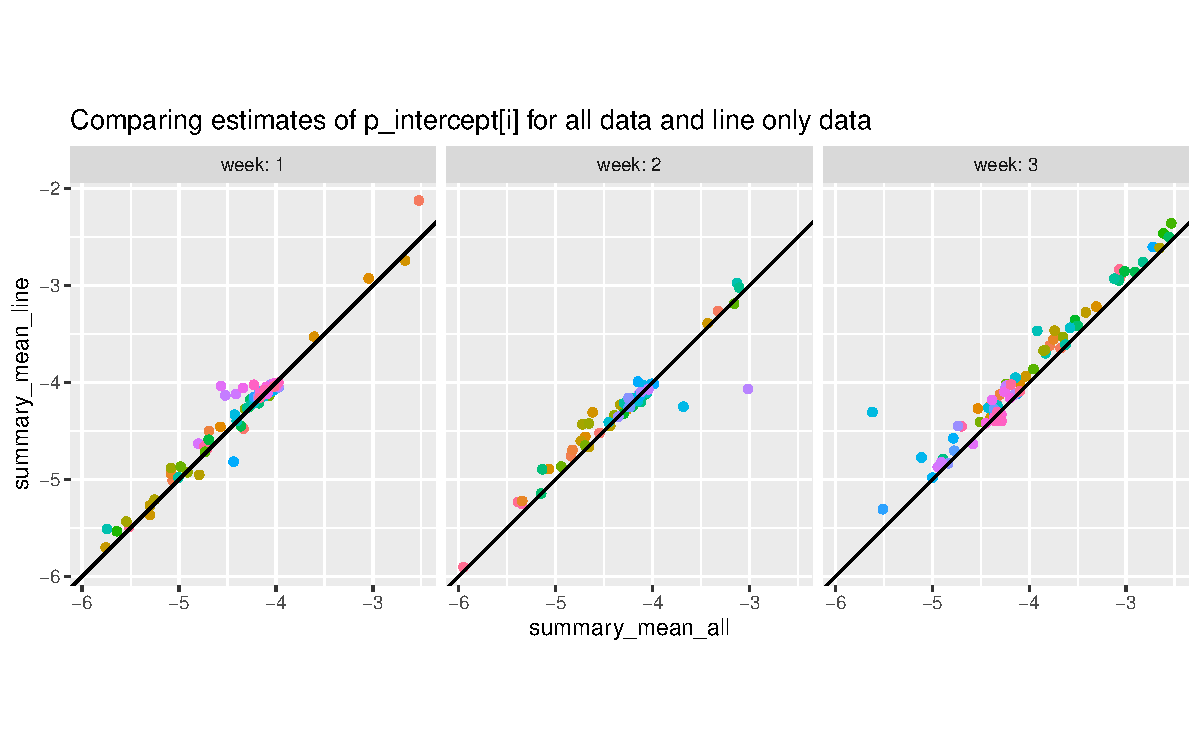
\includegraphics[width=\textwidth]{../visualisations/figures/p_int_est_all_vs_line_data.pdf}
\caption{SD as amount of data increases, depending on \(p\) and the amount of entry data}
\label{fig:SD_est_simulated}
\end{figure}


\begin{table}[ht]
\label{tab:estimates_only_from_all_data}
\caption{Parameter estimates that are only possible when using all data, as opposed to the line-only fits}
\centering
\begin{tabular}{rlrrrr}
  \hline
 & param\_name & week & summary\_mean\_all & summary\_sd\_all & summary\_rhat\_all \\ 
  \hline
1 & p\_intercept[72] & 1.00 & -1.70 & 1.68 & 1.00 \\ 
  2 & p\_intercept[59] & 2.00 & -1.34 & 1.71 & 1.01 \\ 
  3 & p\_intercept[60] & 2.00 & -2.07 & 1.63 & 1.04 \\ 
  4 & p\_intercept[61] & 2.00 & -1.18 & 1.92 & 1.00 \\ 
  5 & country\_effect[62] & 2.00 & -0.01 & 0.49 & 1.00 \\ 
  6 & country\_effect[63] & 2.00 & -0.01 & 0.47 & 1.00 \\ 
  7 & country\_effect[64] & 2.00 & -0.01 & 0.49 & 1.01 \\ 
  8 & country\_effect[65] & 2.00 & 0.02 & 0.48 & 1.02 \\ 
  9 & country\_effect[66] & 2.00 & 0.01 & 0.48 & 1.00 \\ 
  10 & country\_effect[67] & 2.00 & -0.01 & 0.48 & 1.00 \\ 
  11 & p\_intercept[72] & 3.00 & -1.43 & 1.78 & 1.00 \\ 
   \hline
\end{tabular}
\end{table}

\section{Appendix}


\begin{figure}[h!]
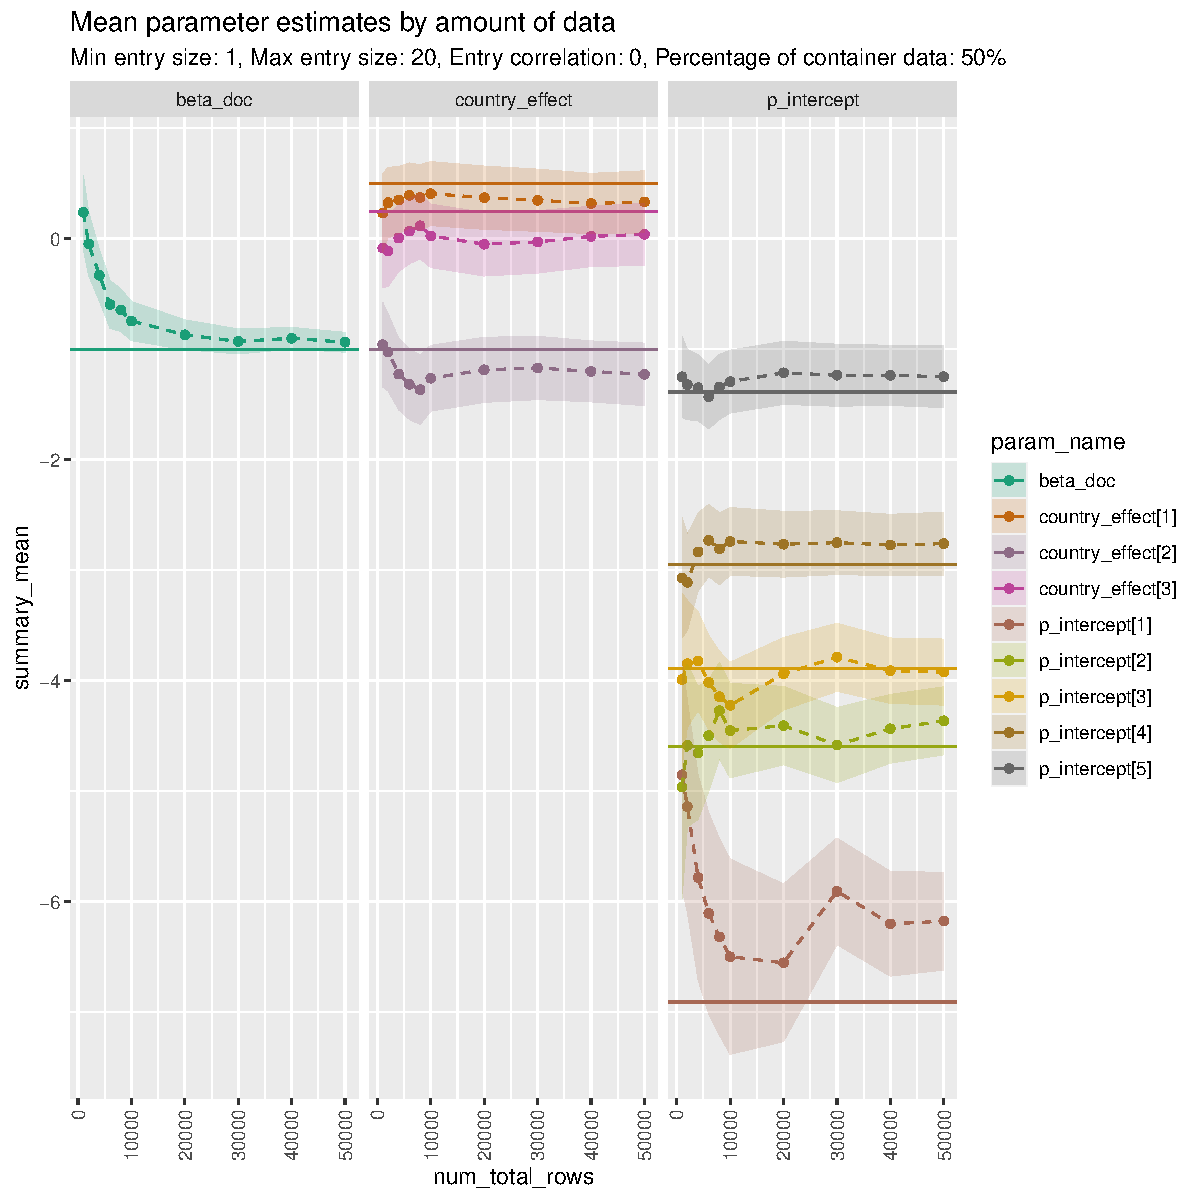
\includegraphics[width=\textwidth]{../visualisations/figures/simulation_estimates.pdf}
\caption{SUPPLEMENT FIGURE}
\label{fig:simulation_estimation}
\end{figure}


\begin{figure}[h!]
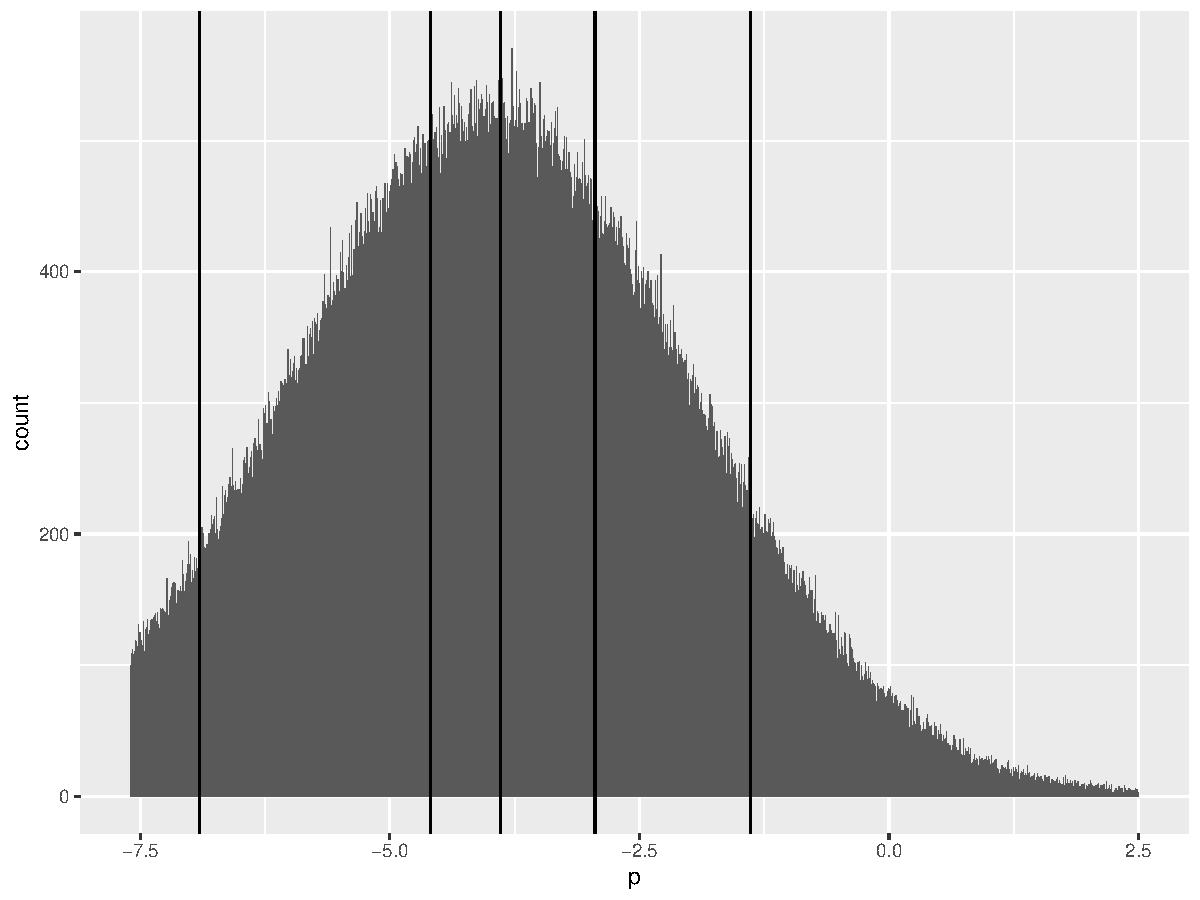
\includegraphics[width=\textwidth]{../visualisations/figures/pint_prior.pdf}
\caption{SUPPLEMENT FIGURE}
\label{fig:p_int_prior}
\end{figure}



%%\begin{figure}[h!]
%%\includegraphics[width=\textwidth]{../results/container_only_stan_vs_SE_est.pdf}
%%\caption{Comparison between SE est and STAN output. The solid black line is the \(y=x\) diagonal, showing when the approximation and STAN outputs match. The points with high SD/SE correspond to fewer entries (i.e. less data).}
%%\label{fig:SE_est_vs_STAN}
%%\end{figure}
%
%\subsubsection{Model accuracy}
%
%To verify that the code works as intended, we generate 100,000 rows of data, and the STAN summary is given in Table~\ref{table:example_stan_output}.
%
%% latex table generated in R 4.0.5 by xtable 1.8-4 package
%% Wed May 19 17:23:26 2021
%\begin{table}[ht]
%\caption{STAN output with 100,000 rows of data. True value is the value is in the simulation, compare it to with either mean or 50\%. Rhat less than 1.1 shows convergence, neff is the stan estimate of effective sample size of the mcmc chains. }
%\label{table:example_stan_output}
%\centering
%\begin{tabular}{clrrrrrrr}
%  \toprule
%True value & Parameter & Rhat & n\_eff & mean & sd & 2.5\% & 50\% & 97.5\% \\ 
%  \midrule
%.01&p[1] & 1.00 & 28798 & 0.01 & 0.00 & 0.01 & 0.01 & 0.02 \\ 
%.05 & p[2] & 1.00 & 30081 & 0.05 & 0.00 & 0.04 & 0.05 & 0.06 \\ 
%.1 & p[3] & 1.00 & 30826 & 0.09 & 0.01 & 0.08 & 0.09 & 0.10 \\ 
%.2 & p[4] & 1.00 & 27377 & 0.21 & 0.01 & 0.19 & 0.21 & 0.23 \\ 
%.5 & p[5] & 1.00 & 30099 & 0.51 & 0.01 & 0.49 & 0.51 & 0.52 \\ 
%.7 & p[6] & 1.00 & 28427 & 0.70 & 0.01 & 0.68 & 0.70 & 0.71 \\ 
%.9 & p[7] & 1.00 & 28211 & 0.90 & 0.01 & 0.89 & 0.90 & 0.91 \\ 
%.95 & p[8] & 1.00 & 28598 & 0.95 & 0.00 & 0.94 & 0.95 & 0.96 \\ 
%-1 & beta\_doc & 1.00 & 23991 & -1.03 & 0.05 & -1.13 & -1.03 & -0.92 \\ 
%
%   \bottomrule
%\end{tabular}
%\end{table}
%
%
%
%\section{Precision and data}
%\subsection{Full model precision}
%Here we investigate how the precision of estimates depend on the type and amount of data used. The three main variables are entry size, mode and number of rows. We generate simulated data sets with the entry size for every entry set to either 2, 3, 4 or 5. For mode, we fit either only the entry data, only the line data, all (ie a random mix of entry and line). Finally, we also vary the number of rows, from 1,000 up to 32,000.
%
%Figure~\ref{fig:line_entry_comparison} shows the difference in the standard deviation of estimate for p2 and entry size 3 by data type, showing line only data has the best precision, followed by all and finally by entry mode. 
%
%
%\begin{figure}[ht]
%\includegraphics[width=\textwidth]{../results/num_rows_by_data_typep[2]containersize3.pdf}
%\caption{Comparison between line/entry/all. Note `entry size' should actually be `entry size'.}
%\label{fig:line_entry_comparison}
%\end{figure}
%
%To see how combining entry and line data changes the standard error, we fit the model using \(n\) rows of line mode data; \(n\) rows of entry mode data; and then we combine these to make a `combined' dataset with \(n+n\) rows. Figure~\ref{fig:facet_plot_entry_size_p1to4} shows the results for various entry sizes and for p[1], p[2], p[3] and p[4]. The horisontal axis is \(n\), meaning that for each point, the combined data set has twice as much data compared to entry or line mode.
%
%\begin{figure}[ht]
%\includegraphics[width=\textwidth]{../results/data_type_comparison_combined_facet.pdf}
%\caption{Comparison between line/entry/all}
%\label{fig:facet_plot_entry_size_p1to4}
%\end{figure}
%
%Next, rather than comparing n line with n entry and n+n line and entry, compare n line with a combination of n line + m*n entry, where m is a multiplyer.Figure \ref{fig:facet_plot_entry_multiplyer_1_3}
%\begin{figure}[ht]
%\includegraphics[width=\textwidth]{../results/container_multiplyer_facet_more_reduced.pdf}
%\caption{Comparison between line and combination}
%\label{fig:facet_plot_entry_multiplyer_1_3}
%\end{figure}
%
%\section{Real data}
%% latex table generated in R 4.0.5 by xtable 1.8-4 package
%% Mon Sep 06 16:40:06 2021
%\begin{table}[ht]
%\centering
%\begin{tabular}{rrrrrr}
%  \hline
% & Broker.key & n\_line & n\_entry & perc\_line\_int & perc\_cont\_int \\ 
%  \hline
%1 & 59216.00 &  53 &   7 & 0.09 & 0.57 \\ 
%  2 & 150563.00 &  29 &  14 & 0.17 & 0.36 \\ 
%  3 & 136950.00 &  25 &   9 & 0.12 & 0.33 \\ 
%  4 & 115644.00 & 161 &  10 & 0.12 & 0.30 \\ 
%  5 & 97131.00 &  28 &  10 & 0.07 & 0.20 \\ 
%  6 & 24737.00 &  45 &   6 & 0.18 & 0.17 \\ 
%  7 & 107590.00 &   9 &   6 & 0.22 & 0.17 \\ 
%  8 & 92303.00 &  31 &   7 & 0.03 & 0.14 \\ 
%  9 & 158922.00 &  45 &   7 & 0.16 & 0.14 \\ 
%  10 & 109007.00 & 265 &  15 & 0.10 & 0.13 \\ 
%  11 & 36185.00 &  37 &   8 & 0.08 & 0.12 \\ 
%  12 & 60592.00 &   9 &   9 & 0.00 & 0.11 \\ 
%  13 & 133385.00 & 122 &  94 & 0.09 & 0.11 \\ 
%  14 & 137511.00 &  15 &  10 & 0.00 & 0.10 \\ 
%  15 & 165467.00 &  31 &  10 & 0.06 & 0.10 \\ 
%  16 & 43377.00 &  65 &  13 & 0.09 & 0.08 \\ 
%  17 & 132068.00 &  41 &  16 & 0.05 & 0.06 \\ 
%  18 & 133658.00 &  36 &  20 & 0.03 & 0.05 \\ 
%  19 & 38439.00 &  53 &  99 & 0.09 & 0.04 \\ 
%  20 & 76534.00 & 153 &  59 & 0.02 & 0.03 \\ 
%   \hline
%\end{tabular}
%\end{table}
%
%
%
%We choose a broker that has 8.5k lines of data. 21 types of item and 8 countries. 5k lines are in entry mode and the remainder are in line mode. We exclude any item types from that dataset which have no entry mode data. We fit the model using all the data, the line only data and the entry only data. We show a scatter plot of the estimates of the fixed effects for the entry mode only and the line mode only fits in figure \ref{fig:country_effect_real_lineventry}. We report all of the means and standard deviations in table~\ref{tab:real_data_fit_comparison}.
%
%
%% latex table generated in R 4.0.5 by xtable 1.8-4 package
%% Tue Aug 31 14:37:59 2021
%\begin{table}[ht]
%\caption{The amount of data for each parameter and the estimate and standard deviation for fits using all of the data, only the line data and only the entry data.}
%\label{tab:real_data_fit_comparison}
%\centering
%\begin{tabular}{rrrrrrrrr}
%  \hline
% & num\_line & num\_entry & all\_mean & all\_sd & line\_mean & line\_sd & entry\_mean & entry\_sd \\ 
%  \hline
%p\_intercept[1] & 2442 & 4423 & -5.46 & 0.42 & -4.62 & 0.45 & -6.48 & 0.73 \\ 
%  p\_intercept[2] & 529 & 995 & -6.16 & 0.65 & -5.44 & 0.68 & -5.58 & 0.87 \\ 
%  p\_intercept[3] &   5 &   7 & -2.12 & 1.29 & -1.81 & 1.38 & -1.30 & 1.36 \\ 
%  p\_intercept[4] &   1 &   1 & -1.22 & 1.55 & -0.75 & 1.71 & -1.13 & 1.64 \\ 
%  country\_effect[1] & 636 & 1005 & 1.57 & 0.34 & 1.55 & 0.35 & -0.14 & 0.47 \\ 
%  country\_effect[2] & 855 & 1642 & -0.79 & 0.39 & -0.73 & 0.42 & -0.19 & 0.46 \\ 
%  country\_effect[3] & 796 & 1577 & -0.94 & 0.40 & -0.88 & 0.40 & -0.30 & 0.46 \\ 
%  country\_effect[4] & 577 & 1000 & -0.65 & 0.42 & -0.60 & 0.43 & -0.18 & 0.47 \\ 
%  country\_effect[5] & 109 & 202 & -0.19 & 0.46 & -0.16 & 0.47 & -0.11 & 0.48 \\ 
%  country\_effect[6] &   1 &   0 & -0.02 & 0.51 & -0.00 & 0.50 &  &  \\ 
%  country\_effect[7] &   3 &   0 & -0.02 & 0.49 & 0.00 & 0.50 &  &  \\ 
%  beta\_doc & 2527 & 4458 & -0.48 & 0.34 & -0.53 & 0.36 & -0.80 & 0.42 \\ 
%   \hline
%\end{tabular}
%\end{table}
%
%
%
%
%\begin{figure}[ht]
%\includegraphics[width=\textwidth]{../model/P_effect_line_v_entry_scatterplot.pdf}
%\caption{Country effect and doc effect for real data}
%\label{fig:country_effect_real_lineventry}
%\end{figure}

%\section{Simulation code}
%\begin{lstlisting}
%library(tidyverse)
%library(optimx)
%
%simulation_name <- 'entry_line_simulated_data' # A name that is used as part of the save filename
%
%# The true probability of interception of each item type
%true_intercept_probability <- c(.01, .05, .1, .2, .5, .7, .9, .95)
%
%num_types <- length(true_intercept_probability) # number of item types
%
%# probability of inspection. Currently set to 1 so everything is inspects. However,
%# this could be altered in future
%true_inspect_probability <- integer(num_types) + 1
%
%
%prob_line <- 0.25 # probability that an entry is in line mode
%target_num_rows_data <- 100000 # number of rows of data to generate
%
%pr_doc <- .2 # probability that each row of data has documentation
%doc_effect <- 1 # The effect on the probability of interception if there is documetation
%
%
%# A check that the length of the inspect and intercept probability lists are the same
%if (length(true_inspect_probability) != num_types){
%  stop("Inspect and defect probability lists must be the same length")
%}
%
%for (entry_size in c(2,3,4)){
%  # In general, entry size can be a random number
%  max_entry_size <- entry_size
%  min_entry_size <- entry_size
%
%
%  create_row_of_data <- function (doc){
%    # create_row_of_data creates the data for a single row of data
%    item_type <- sample.int(num_types, 1) # The item type is selected randomly
%    item_inspect <- runif(1) < true_inspect_probability[item_type] # Draw whether it is inspected
%    if (item_inspect == TRUE){
%      # If it has documentation, set the current_doc_effect to the true value, otherwise set it to zero
%      if (doc == TRUE){
%        current_doc_effect <- doc_effect
%      } else {
%        current_doc_effect <- 0
%      }
%      # Store the probability of interception. If current_doc_effect is zero, then this line does nothing.
%      # If there is documenation, then the probability of inteception is reduced, using the logistic function
%      current_intercept_pr <- plogis(qlogis(true_intercept_probability[item_type]) - current_doc_effect)
%
%      item_intercept <- runif(1) < current_intercept_pr # Draw whether it was intercepted
%    } else {
%      item_intercept <- FALSE # If not inspected, intercept is false.
%    }
%    return(c(item_type, item_inspect, item_intercept))
%  }
%
%  add_entry_to_df <- function(entry_true_data, mode, line, doc, current_rows, df){
%    # Adds the data for a row to the dataframe
%    if (current_rows == 0){
%      # If the dataframe is empty, then create it
%      # Note, at this stage True and Record are identical, and these are adjusted later, for rows in entry mode.
%      test_data <- data.frame(Type = entry_true_data[1],
%                              Mode=mode,
%                              Entry=current_entry,
%                              Line=line,
%                              Documentation=doc,
%                              TrueInspect=entry_true_data[2],
%                              TrueIntercept=entry_true_data[3],
%                              RecordInspect=entry_true_data[2],
%                              RecordIntercept=entry_true_data[3])
%    } else {
%      test_data <- rbind(df, c(entry_true_data[1], mode, current_entry,line, doc,
%                               entry_true_data[2],
%                               entry_true_data[3],
%                               entry_true_data[2],
%                               entry_true_data[3]))
%    }
%    return(test_data)
%  }
%
%  current_rows <- 0 # Set the num rows of data to zero
%  current_entry <- 1 # Initialise with entry number 1
%  simulated_data <- NULL # Initialise with data = null
%
%  while (current_rows < target_num_rows_data){
%    # Add rows of data until the target number is reached
%    print(c(entry_size, current_rows)) # display current state of loop
%
%    # Draw the entry size, which is the number of rows of data in the entry
%    entry_size <- sample.int(max_entry_size - (min_entry_size - 1), 1) + (min_entry_size - 1)
%
%    # Draw whether the entry is in line or entry mode
%    if (runif(1) < prob_line){
%      mode <- 'Line'
%    } else {
%      mode <- 'Entry'
%    }
%
%    # For the number of rows of data in the entry, create the data and add it to the data frame
%    for (i in 1:entry_size){
%      doc <- runif(1) <pr_doc # Draw whether there is documentaion
%      entry_true_data <- create_row_of_data(doc) # Create the data
%
%      # Add the new row to the dataframe
%      simulated_data <- add_entry_to_df(entry_true_data, mode=mode, line=i,
%                                        doc=doc, current_rows=current_rows, df=simulated_data)
%    }
%
%    if (mode == 'Entry'){
%      # If the entry is in entry mode, if any row of data is inspected, all rows of data are set to inspected.
%      # Similarly, if a row is intercpeted, all rows in the entry is set to intercepted.
%      if (any(simulated_data[simulated_data$Entry == current_entry,]$TrueInspect == 1)){
%        simulated_data[simulated_data$Entry == current_entry,]$RecordInspect <- 1
%        if (any(simulated_data[simulated_data$Entry == current_entry,]$TrueIntercept == 1)){
%          simulated_data[simulated_data$Entry == current_entry,]$RecordIntercept <- 1
%        } 
%      }
%    }
%
%    current_entry <- current_entry + 1 # Increment the entry number
%    current_rows <- nrow(simulated_data) # Update the current number of rows of data.
%  }
%
%  write.csv(simulated_data, paste0('../data/', simulation_name, min_entry_size, '_', max_entry_size,
%                                   '_rows_', target_num_rows_data, '.csv'), row.names = FALSE)
%}
%\end{lstlisting}
\bibliography{entry-line}{}
%\bibliographystyle{plain}
\end{document}